\documentclass[12pt,]{article}
\usepackage[utf8]{inputenc}
\usepackage[T1]{fontenc}
\usepackage{mathptmx}
\usepackage{geometry}
\usepackage{mathtools}
\usepackage[english]{babel}
\usepackage{graphicx}
\usepackage[os=win]{menukeys}
\usepackage[figurename=Gambar]{caption}
\usepackage{hyperref}
\usepackage{minted}
\usepackage{xcolor}
\usepackage{tikz}
\usepackage[yyyymmdd,hhmmss]{datetime}

\newcommand{\ShowOsVersion}{
	\immediate\write18{\unexpanded{foo=`uname -sro` && echo "\\\verb${foo}" > tmp.tex}}
	\input{tmp}\immediate\write18{rm tmp.tex}
}

\newcommand{\ShowTexVersion}{
	\immediate\write18{\unexpanded{foo=`pdflatex -version | head -n1` && echo "\\\verb${foo}" > tmp.tex}}
	\input{tmp}\immediate\write18{rm tmp.tex}
}

\addto\captionsenglish{\renewcommand{\contentsname}{Daftar Isi}}

\hypersetup{
	colorlinks=true, %set true if you want colored links
	linktoc=all,     %set to all if you want both sections and subsections linked
	linkcolor=blue,  %choose some color if you want links to stand out
}

\geometry{
	a4paper,
	left=15mm,
	right=10mm,
	top=10mm,
	bottom=10mm,
}

\title{\Large \bf
	Dokumen Teknis dan Laporan Sementara Development Instrumen PikoAkustik
}

\author{Achmadi ST MT}

\date{}

\definecolor{LightGray}{gray}{0.9}

\usetikzlibrary{trees}

\tikzstyle{every node}=[draw=black,thick,anchor=west]
\tikzstyle{selected}=[draw=red,fill=red!30]

\begin{document}

	\maketitle
	\thispagestyle{empty}
	\pagestyle{empty}
	
	\begin{figure}[!ht]
		\centering
		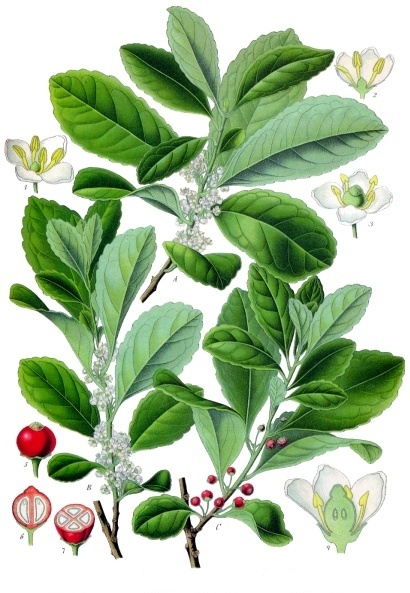
\includegraphics[width=250pt]{images/yerba.png}
	\end{figure}
	
	\vspace*{125px}
	\noindent This report written using: \\
	OS : \ShowOsVersion \\
	TeX : \ShowTexVersion \\
	Update: {\today} at \currenttime \\
	
	\noindent Document Tex Source:\\
	\url{https://github.com/mekatronik-achmadi/hts_grapheme/blob/master/panduan/panduan.tex}
	
	\newpage
	\mbox{}

\end{document}
\tikzstyle{optional}=[dashed,fill=gray!50]
